%!TeX root=../pridetop.tex
\chapter[Chapter \thechapter]{}
	
	\begin{figure}[t!]
\centering
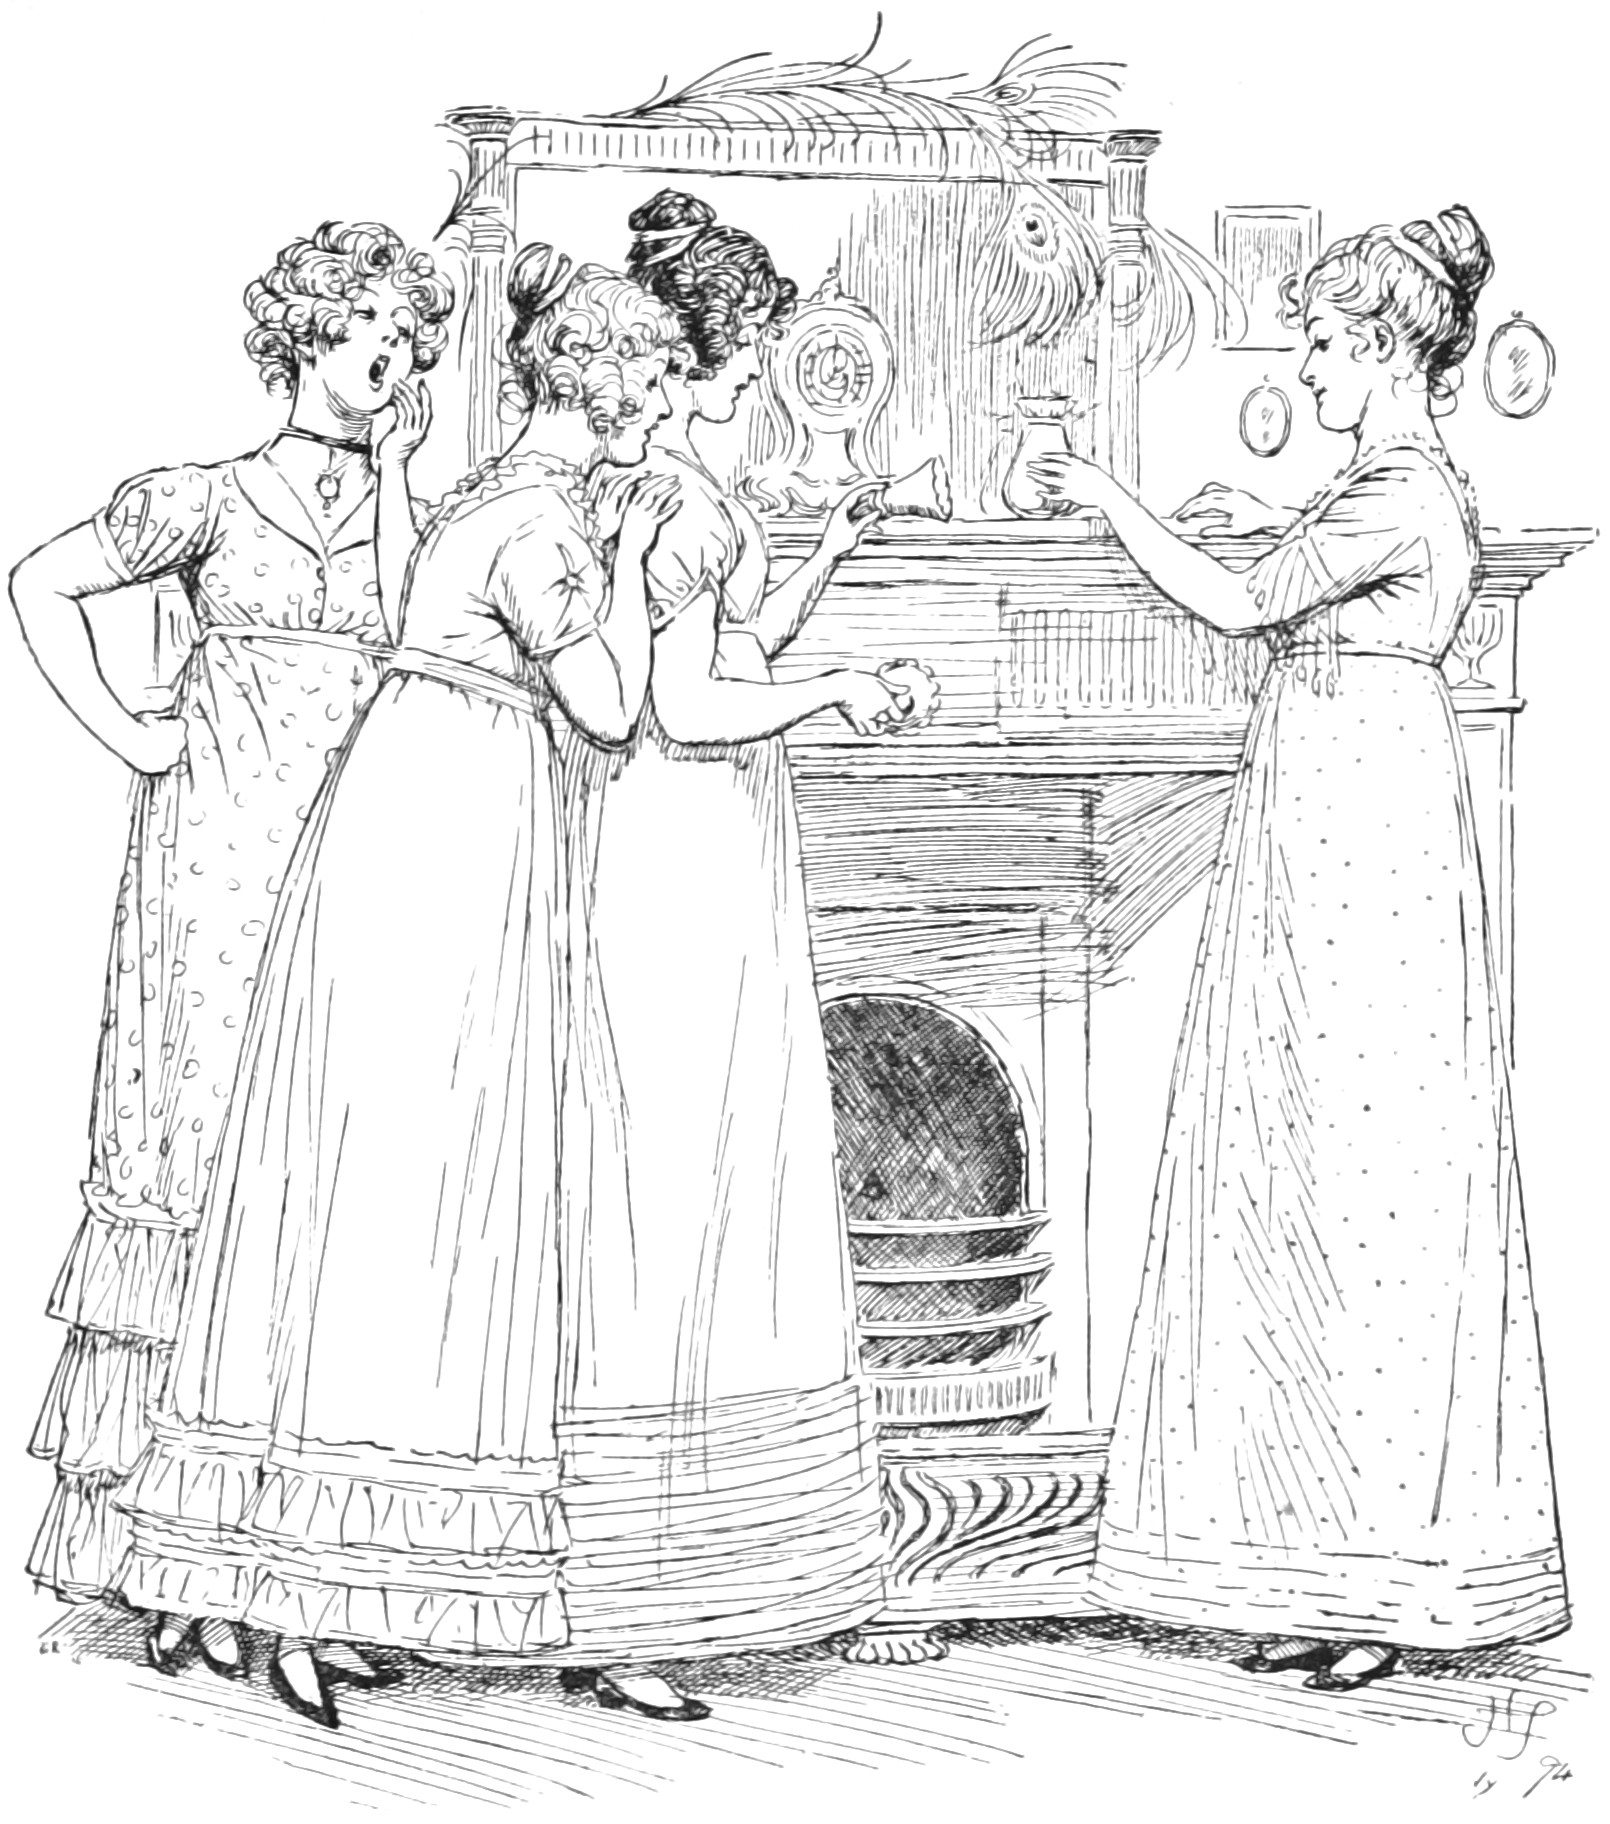
\includegraphics[width=.8\linewidth]{16top}
\captionlistentry{China on the mantel-piece}
\end{figure}

\lettrine[lines=6,image=true,loversize=.18]{initials/chap16a}{s}  no objection was made to the young people's engagement with their aunt, and all Mr Collins's scruples of leaving Mr and Mrs Bennet for a single evening during his visit were most steadily resisted, the coach conveyed him and his five cousins at a suitable hour to Meryton; and the girls had the pleasure of hearing, as they entered the drawing-room, that Mr Wickham had accepted their uncle's invitation, and was then in the house.

When this information was given, and they had all taken their seats, Mr Collins was at leisure to look around him and admire, and he was so much struck with the size and furniture of the apartment, that he declared he might almost have supposed himself in the small summer breakfast parlour at Rosings; a comparison that did not at first convey much gratification; but when Mrs Philips understood from him what Rosings was, and who was its proprietor, when she had listened to the description of only one of Lady Catherine's drawing-rooms, and found that the chimney-piece alone had cost eight hundred pounds, she felt all the force of the compliment, and would hardly have resented a comparison with the housekeeper's room.



In describing to her all the grandeur of Lady Catherine and her mansion, with occasional digressions in praise of his own humble abode, and the improvements it was receiving, he was happily employed until the gentlemen joined them; and he found in Mrs Philips a very attentive listener, whose opinion of his consequence increased with what she heard, and who was resolving to retail it all among her neighbours as soon as she could. To the girls, who could not listen to their cousin, and who had nothing to do but to wish for an instrument, and examine their own indifferent imitations of china on the mantel-piece, the interval of waiting appeared very long. It was over at last, however. The gentlemen did approach: and when Mr Wickham walked into the room, Elizabeth felt that she had neither been seeing him before, nor thinking of him since, with the smallest degree of unreasonable admiration. The officers of the ⸺shire were in general a very creditable, gentlemanlike set and the best of them were of the present party; but Mr Wickham was as far beyond them all in person, countenance, air, and walk, as \textit{they} were superior to the broad-faced stuffy uncle Philips, breathing port wine, who followed them into the room.

\begin{figure}[tbh]
\centering

\includegraphics[width=.8\linewidth]{16officers}
\captionlistentry{The officers of the ⸺shire}
\end{figure}


Mr Wickham was the happy man towards whom almost every female eye was turned, and Elizabeth was the happy woman by whom he finally seated himself; and the agreeable manner in which he immediately fell into conversation, though it was only on its being a wet night, and on the probability of a rainy season, made her feel that the commonest, dullest, most threadbare topic might be rendered interesting by the skill of the speaker.

With such rivals for the notice of the fair as Mr Wickham and the officers, Mr Collins seemed to sink into insignificance; to the young ladies he certainly was nothing; but he had still at intervals a kind listener in Mrs Philips, and was, by her watchfulness, most abundantly supplied with coffee and muffin.

When the card tables were placed, he had an opportunity of obliging her, in return, by sitting down to whist.

<I know little of the game at present,> said he, <but I shall be glad to improve myself; for in my situation of life\longdash> Mrs Philips was very thankful for his compliance, but could not wait for his reason.

Mr Wickham did not play at whist, and with ready delight was he received at the other table between Elizabeth and Lydia. At first there seemed danger of Lydia's engrossing him entirely, for she was a most determined talker; but being likewise extremely fond of lottery tickets, she soon grew too much interested in the game, too eager in making bets and exclaiming after prizes, to have attention for anyone in particular. Allowing for the common demands of the game, Mr Wickham was therefore at leisure to talk to Elizabeth, and she was very willing to hear him, though what she chiefly wished to hear she could not hope to be told, the history of his acquaintance with Mr Darcy. She dared not even mention that gentleman. Her curiosity, however, was unexpectedly relieved. Mr Wickham began the subject himself. He inquired how far Netherfield was from Meryton; and, after receiving her answer, asked in a hesitating manner how long Mr Darcy had been staying there.

<About a month,> said Elizabeth; and then, unwilling to let the subject drop, added, <he is a man of very large property in Derbyshire, I understand.>

<Yes,> replied Wickham; <his estate there is a noble one. A clear ten thousand per annum. You could not have met with a person more capable of giving you certain information on that head than myself—for I have been connected with his family, in a particular manner, from my infancy.>

Elizabeth could not but look surprised.

<You may well be surprised, Miss Bennet, at such an assertion, after seeing, as you probably might, the very cold manner of our meeting yesterday. Are you much acquainted with Mr Darcy?>

<As much as I ever wish to be,> cried Elizabeth, warmly. <I have spent four days in the same house with him, and I think him very disagreeable.>

<I have no right to give \textit{my} opinion,> said Wickham, <as to his being agreeable or otherwise. I am not qualified to form one. I have known him too long and too well to be a fair judge. It is impossible for \textit{me} to be impartial. But I believe your opinion of him would in general astonish—and, perhaps, you would not express it quite so strongly anywhere else. Here you are in your own family.>

<Upon my word I say no more \textit{here} than I might say in any house in the neighbourhood, except Netherfield. He is not at all liked in Hertfordshire. Everybody is disgusted with his pride. You will not find him more favourably spoken of by anyone.>

<I cannot pretend to be sorry,> said Wickham, after a short interruption, <that he or that any man should not be estimated beyond their deserts; but with \textit{him} I believe it does not often happen. The world is blinded by his fortune and consequence, or frightened by his high and imposing manners, and sees him only as he chooses to be seen.>

<I should take him, even on \textit{my} slight acquaintance, to be an ill-tempered man.>

Wickham only shook his head.

<I wonder,> said he, at the next opportunity of speaking, <whether he is likely to be in this country much longer.>

<I do not at all know; but I \textit{heard} nothing of his going away when I was at Netherfield. I hope your plans in favour of the ⸺shire will not be affected by his being in the neighbourhood.>

<Oh no—it is not for \textit{me} to be driven away by Mr Darcy. If \textit{he} wishes to avoid seeing \textit{me} he must go. We are not on friendly terms, and it always gives me pain to meet him, but I have no reason for avoiding \textit{him} but what I might proclaim to all the world—a sense of very great ill-usage, and most painful regrets at his being what he is. His father, Miss Bennet, the late Mr Darcy, was one of the best men that ever breathed, and the truest friend I ever had; and I can never be in company with this Mr Darcy without being grieved to the soul by a thousand tender recollections. His behaviour to myself has been scandalous; but I verily believe I could forgive him anything and everything, rather than his disappointing the hopes and disgracing the memory of his father.>

Elizabeth found the interest of the subject increase, and listened with all her heart; but the delicacy of it prevented further inquiry.

Mr Wickham began to speak on more general topics, Meryton, the neighbourhood, the society, appearing highly pleased with all that he had yet seen, and speaking of the latter, especially, with gentle but very intelligible gallantry.

<It was the prospect of constant society, and good society,> he added, <which was my chief inducement to enter the ⸺shire. I know it to be a most respectable, agreeable corps; and my friend Denny tempted me further by his account of their present quarters, and the very great attentions and excellent acquaintance Meryton had procured them. Society, I own, is necessary to me. I have been a disappointed man, and my spirits will not bear solitude. I \textit{must} have employment and society. A military life is not what I was intended for, but circumstances have now made it eligible. The church \textit{ought} to have been my profession—I was brought up for the church; and I should at this time have been in possession of a most valuable living, had it pleased the gentleman we were speaking of just now.>

<Indeed!>

<Yes—the late Mr Darcy bequeathed me the next presentation of the best living in his gift. He was my godfather, and excessively attached to me. I cannot do justice to his kindness. He meant to provide for me amply, and thought he had done it; but when the living fell, it was given elsewhere.>

<Good heavens!> cried Elizabeth; <but how could \textit{that} be? How could his will be disregarded? Why did not you seek legal redress?>

<There was just such an informality in the terms of the bequest as to give me no hope from law. A man of honour could not have doubted the intention, but Mr Darcy chose to doubt it—or to treat it as a merely conditional recommendation, and to assert that I had forfeited all claim to it by extravagance, imprudence, in short, anything or nothing. Certain it is that the living became vacant two years ago, exactly as I was of an age to hold it, and that it was given to another man; and no less certain is it, that I cannot accuse myself of having really done anything to deserve to lose it. I have a warm unguarded temper, and I may perhaps have sometimes spoken my opinion \textit{of} him, and \textit{to} him, too freely. I can recall nothing worse. But the fact is, that we are very different sort of men, and that he hates me.>

<This is quite shocking! He deserves to be publicly disgraced.>

<Some time or other he \textit{will} be—but it shall not be by \textit{me}. Till I can forget his father, I can never defy or expose \textit{him}.>

Elizabeth honoured him for such feelings, and thought him handsomer than ever as he expressed them.

<But what,> said she, after a pause, <can have been his motive? what can have induced him to behave so cruelly?>

<A thorough, determined dislike of me—a dislike which I cannot but attribute in some measure to jealousy. Had the late Mr Darcy liked me less, his son might have borne with me better; but his father's uncommon attachment to me irritated him, I believe, very early in life. He had not a temper to bear the sort of competition in which we stood—the sort of preference which was often given me.>

<I had not thought Mr Darcy so bad as this—though I have never liked him, I had not thought so very ill of him—I had supposed him to be despising his fellow-creatures in general, but did not suspect him of descending to such malicious revenge, such injustice, such inhumanity as this!>

After a few minutes' reflection, however, she continued, <I \textit{do} remember his boasting one day, at Netherfield, of the implacability of his resentments, of his having an unforgiving temper. His disposition must be dreadful.>

<I will not trust myself on the subject,> replied Wickham; <\textit{I} can hardly be just to him.>

Elizabeth was again deep in thought, and after a time exclaimed, <To treat in such a manner the godson, the friend, the favourite of his father!> She could have added, <A young man, too, like \textit{you}, whose very countenance may vouch for your being amiable.> But she contented herself with—<And one, too, who had probably been his own companion from childhood, connected together, as I think you said, in the closest manner.>

<We were born in the same parish, within the same park; the greatest part of our youth was passed together: inmates of the same house, sharing the same amusements, objects of the same parental care. \textit{My} father began life in the profession which your uncle, Mr Philips, appears to do so much credit to; but he gave up everything to be of use to the late Mr Darcy, and devoted all his time to the care of the Pemberley property. He was most highly esteemed by Mr Darcy, a most intimate, confidential friend. Mr Darcy often acknowledged himself to be under the greatest obligations to my father's active superintendence; and when, immediately before my father's death, Mr Darcy gave him a voluntary promise of providing for me, I am convinced that he felt it to be as much a debt of gratitude to \textit{him} as of affection to myself.>

<How strange!> cried Elizabeth. <How abominable! I wonder that the very pride of this Mr Darcy has not made him just to you. If from no better motive, that he should not have been too proud to be dishonest,—for dishonesty I must call it.>

<It \textit{is} wonderful,> replied Wickham; <for almost all his actions may be traced to pride; and pride has often been his best friend. It has connected him nearer with virtue than any other feeling. But we are none of us consistent; and in his behaviour to me there were stronger impulses even than pride.>

<Can such abominable pride as his have ever done him good?>

<Yes; it has often led him to be liberal and generous; to give his money freely, to display hospitality, to assist his tenants, and relieve the poor. Family pride, and \textit{filial} pride, for he is very proud of what his father was, have done this. Not to appear to disgrace his family, to degenerate from the popular qualities, or lose the influence of the Pemberley House, is a powerful motive. He has also \textit{brotherly} pride, which, with \textit{some} brotherly affection, makes him a very kind and careful guardian of his sister; and you will hear him generally cried up as the most attentive and best of brothers.>

<What sort of a girl is Miss Darcy?>

He shook his head. <I wish I could call her amiable. It gives me pain to speak ill of a Darcy; but she is too much like her brother,—very, very proud. As a child, she was affectionate and pleasing, and extremely fond of me; and I have devoted hours and hours to her amusement. But she is nothing to me now. She is a handsome girl, about fifteen or sixteen, and, I understand, highly accomplished. Since her father's death her home has been London, where a lady lives with her, and superintends her education.>

After many pauses and many trials of other subjects, Elizabeth could not help reverting once more to the first, and saying,—

<I am astonished at his intimacy with Mr Bingley. How can Mr Bingley, who seems good-humour itself, and is, I really believe, truly amiable, be in friendship with such a man? How can they suit each other? Do you know Mr Bingley?>

<Not at all.>

<He is a sweet-tempered, amiable, charming man. He cannot know what Mr Darcy is.>

<Probably not; but Mr Darcy can please where he chooses. He does not want abilities. He can be a conversible companion if he thinks it worth his while. Among those who are at all his equals in consequence, he is a very different man from what he is to the less prosperous. His pride never deserts him; but with the rich he is liberal-minded, just, sincere, rational, honourable, and, perhaps, agreeable,—allowing something for fortune and figure.>

The whist party soon afterwards breaking up, the players gathered round the other table, and Mr Collins took his station between his cousin Elizabeth and Mrs Philips. The usual inquiries as to his success were made by the latter. It had not been very great; he had lost every point; but when Mrs Philips began to express her concern thereupon, he assured her, with much earnest gravity, that it was not of the least importance; that he considered the money as a mere trifle, and begged she would not make herself uneasy.

<I know very well, madam,> said he, <that when persons sit down to a card table they must take their chance of these things,—and happily I am not in such circumstances as to make five shillings any object. There are, undoubtedly, many who could not say the same; but, thanks to Lady Catherine de Bourgh, I am removed far beyond the necessity of regarding little matters.>

Mr Wickham's attention was caught; and after observing Mr Collins for a few moments, he asked Elizabeth in a low voice whether her relations were very intimately acquainted with the family of de Bourgh.

<Lady Catherine de Bourgh,> she replied, <has very lately given him a living. I hardly know how Mr Collins was first introduced to her notice, but he certainly has not known her long.>

<You know of course that Lady Catherine de Bourgh and Lady Anne Darcy were sisters; consequently that she is aunt to the present Mr Darcy.>

<No, indeed, I did not. I knew nothing at all of Lady Catherine's connections. I never heard of her existence till the day before yesterday.>

<Her daughter, Miss de Bourgh, will have a very large fortune, and it is believed that she and her cousin will unite the two estates.>

This information made Elizabeth smile, as she thought of poor Miss Bingley. Vain indeed must be all her attentions, vain and useless her affection for his sister and her praise of himself, if he were already self-destined to another.

<Mr Collins,> said she, <speaks highly both of Lady Catherine and her daughter; but, from some particulars that he has related of her Ladyship, I suspect his gratitude misleads him; and that, in spite of her being his patroness, she is an arrogant, conceited woman.>

<I believe her to be both in a great degree,> replied Wickham; <I have not seen her for many years; but I very well remember that I never liked her, and that her manners were dictatorial and insolent. She has the reputation of being remarkably sensible and clever; but I rather believe she derives part of her abilities from her rank and fortune, part from her authoritative manner, and the rest from the pride of her nephew, who chooses that everyone connected with him should have an understanding of the first class.>

Elizabeth allowed that he had given a very rational account of it, and they continued talking together with mutual satisfaction till supper put an end to cards, and gave the rest of the ladies their share of Mr Wickham's attentions. There could be no conversation in the noise of Mrs Philips's supper party, but his manners recommended him to everybody. Whatever he said, was said well; and whatever he did, done gracefully. Elizabeth went away with her head full of him. She could think of nothing but of Mr Wickham, and of what he had told her, all the way home; but there was not time for her even to mention his name as they went, for neither Lydia nor Mr Collins were once silent. Lydia talked incessantly of lottery tickets, of the fish she had lost and the fish she had won; and Mr Collins, in describing the civility of Mr and Mrs Philips, protesting that he did not in the least regard his losses at whist, enumerating all the dishes at supper, and repeatedly fearing that he crowded his cousins, had more to say than he could well manage before the carriage stopped at Longbourn House.